\documentclass[11pt]{article}
\usepackage{geometry}
\frenchspacing
\usepackage{graphicx}
\usepackage{amsmath,amssymb,latexsym}
\usepackage{lscape}
\usepackage{textgreek}

\begin{document}

{\huge
\begin{center}
\textbf{EE 119c Proposal: LMS Adaptive FIR filter for 16-QAM}
\

\


\textbf{Harrison Krowas}
\

\
\end{center}
}

\section{Functional Specification}

This project is to implement an LMS error, decision-directed adaptive FIR filter for 16-QAM. The filter presented in \cite{kikuchi} will be exactly implemented, and such filters are used to correct for the dispersive effects of fiber transmission.

The filter itself is a standard FIR filter with adjustable tap coefficients, and the number of taps is a generic. The error computation unit is used to control the value of the tap coefficients based on the LMS error. The coefficients are updated on every time step according to the following formula
\[
\vec{c}(n + 1) = \vec{c}(n) + \mu e(n) \vec{E}_{in}(n)^{*}\cite{kikuchi}
\]
\[
e(n) = d(n) - \vec{E}_{out}(n)\cite{kikuchi}
\]
where $d(n)$ is the point in the 16-QAM constellation that is closest to $\vec{E}_{out}(n)$.

The filter operates on 16-bit data. Each tap of the FIR filter is implemented using fully parallelized multiplier array, so that the computation can be performed in one clock. The summation is also performed entirely in parallel.

The error computation unit feeds back into the filter changing the tap coefficients on every clock according to the error.

In total, it takes a single clock to process each input symbol. The max data rate is then $4 \times f$ b/s, where f is the system frequency.

\begin{figure}
\begin{center}
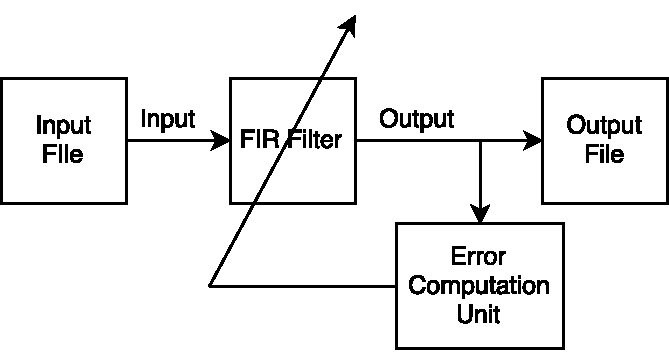
\includegraphics{adaptive_filter_block_diagram}
\caption{Complete system block diagram. Input data is from a file, is passed through the filter, the error computation unit feeds back into the filter changing the tap coefficients, and the output data is written to a file.}
\end{center}
\end{figure}

\begin{figure}
\begin{center}
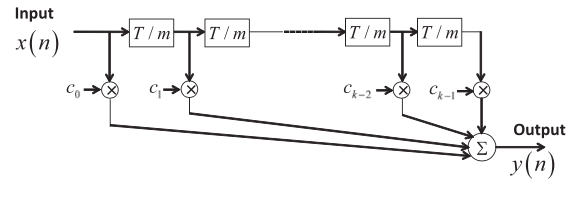
\includegraphics[scale = 0.5]{fir_filter}
\caption{FIR filter topology. The tap coefficients, $c_n$, are variable.\cite{kikuchi}}
\end{center}
\end{figure}

\section{Demonstration}

The system is demonstrated by creating random input data, modulating it into a series of 16-QAM points, passing it through some filter to simulate the effects of fiber transmission (such as a Gaussian filter), and saving it to an input file. The points from this input file are read into the adaptive filter, one per clock. The output of the filter is saved into a file.

The quality of the resulting output data can be checked quantitatively by comparing it to the input data. If it is the same, then the filter was able to remove the channel impairments. Another metric, called error vector magnitude (EVM), is determined by measuring the distance from each output point to its corresponding point on the 16-QAM constellation.

\section{Schedule}

Weeks 2 and 3: High level implementation completed.\\
Week 4: Complex multiplier entity completed and tested.
Week 5: The high-level hardware design is completed and low-level implementation has begun. Detailed block diagrams along with the implementation for those parts of the design implemented.\\
Week 6: Complex adder entity completed and tested. Error computation unit completed and tested.\\
Week 7: System test bench code completed.\\
Week 8: The low-level implementation mostly done and testing started. Able to show a complete design and demonstrate portions of the design using a simulator.\\
Week 9: Optimization for speed. Filter has been tested and results (error rate and EVM) are acquired.\\

\begin{thebibliography}{20}

\bibitem{kikuchi} Kikuchi, K. ``Fundamentals of Coherent Optical Fiber Communications.'' Journal of Lightwave Technology 34, 1 (January 2016)\: 157--179.

\end{thebibliography}

\end{document}
